%%%%%%%%%%%%%%%%%%%%%%%%%%%%%%%%%%%%%%%%%%%%%%%%%%%%%%%%%%%%%%%%%%%%%%%%%%%%%%%%%%%%%%%%%%%%%%%%%%%%%%%%%%%%%%%%%%%%%%%%%%%%%%%%%%%%%%%%%%%%
%%%%%%%%%%%%%%%%%%%%%%%%%%%%%%%%%%%%%%%%%%%%%%%%%%%%%%%%%%%%%%%%%%%%%%%%%%%%%%%%%%%%%%%%%%%%%%%%%%%%%%%%%%%%%%%%%%%%%%%%%%%%%%%%%%%%%%%%%%%%
% Dies ist ein Kommentar, er wird bei der pdf-Erzeugung ignoriert.


% Dies ist eine LaTex-Vorlage für den Gebrauch im Physikalischen Praktikum I und ist als Hilfestellung zu verstehen, falls keine LaTex-Kenntnisse vorhanden sind. Einige nötige und nützliche Pakete sind bereits eingebunden und die Kapitel (\section) angelegt. Die Kapitel beinhalten teilweise Beispiele wie die Darstellung von Grafiken/Tabellen oder mathematischen Formeln sowie Referenzen/Zitationen. Nach den nun folgenden Paketeinbindungen und Definitionen können die Namen der Verfasser, der Versuchsname usw. eingegeben werden. 


%%%%%%%%%%%%%%%%%%%%%%%%%%%%%%%%%%%%%%%%%%%%%%%%%%%%%%%%%%%%%%%%%%%%%%%%%%%%%%%%%%%%%%%%%%%%%%%%%%%%%%%%%%%%%%%%%%%%%%%%%%%%%%%%%%%%%%%%%%%%
%%%%%%%%%%%%%%%%%%%%%%%%%%%%%%%%%%%%%%%%%%%%%%%%%%%%%%%%%%%%%%%%%%%%%%%%%%%%%%%%%%%%%%%%%%%%%%%%%%%%%%%%%%%%%%%%%%%%%%%%%%%%%%%%%%%%%%%%%%%%
\documentclass[a4paper,12pt,bibtotocnumbered]{scrartcl}

\usepackage[utf8]{inputenc} %Codierung des LaTeX-Dokumentes. Auf Windows-Maschinen ist statt utf8 auch ANSIC als Codierung möglich, aber unnötig, da utf8 in jeder Hinsicht besser als ANSI ist. Bei Linux: latin1 als Codierung, auf MacOS X: applemac
\usepackage[T1]{fontenc}
\usepackage[ngerman]{babel} %Deutsche Zeichen- und Umbruchsetzung
\usepackage{amsmath, amssymb,amsfonts} %AMS-TeX-Pakete. Nötig für die Definition der Mathematik-Umgebung
\usepackage{graphicx} %Nötig, um Grafiken einbinden zu können
\usepackage[bookmarks,colorlinks=true]{hyperref} %Mittels hyperref lassen sich hyperlinks innerhalb des PDF-Dokumentes benutzen. Beispiel: Mausklick im Inhaltsverzeichnis auf ein Kapitel führt zum automatischen Sprung in dieses Kapitel
\usepackage{geometry}
\usepackage{float}
%Ein Paket, mit dem sich ohne Probleme mehrseitige PDF-Dokumente ohne \includegraphics-Rumgemache einbinden lassen. Befehl: \includepdf[pages=a-b]{PDFfile.pdf}. Einzelne Seiten, oder auch alle Seiten (Option pages=-) können angewählt werden
%Wenn keine Option angegeben wird, gilt pages=1!
\usepackage[final]{pdfpages}
\usepackage{framed, color} %Framed: Paket, mittels dessen ein Rahmen um einen Bereich definiert werden kann. Color: Lässt Farbdarstellung in Schrift, Hintergrund etc. zu
\usepackage{scrlayer-scrpage} %Header für die KOMA-script -Klasse
\usepackage{siunitx} %Ein schönes Paket, um Einheiten und physikalische Größen richtig zu setzen. Z.B.  \SI{2}{\kilo\gram\per\meter\squared}
\usepackage[square,numbers]{natbib}
\usepackage{subfigure} %Mehrere Bilder in einer Figure-Umgebung
\usepackage{lipsum}  


%siunitx-Konfiguration. Damit werden die richtigen Font-Einstellungen erkannt (also beispielsweise fett, kursiv etc.) und damit  ebenfalls die deutsche Zeichensetzung, insbesondere Trennungszeichen, benutzt werden. 
%Ebenso wird bei SIrange das "`to"' in "`bis"' umgewandelt, bei SIlist das "`and"' in "`und"'
\sisetup{detect-weight=true, detect-family=true,locale=DE,range-phrase={\,bis\,},list-final-separator ={\,\linebreak[0] \text{und}\,},separate-uncertainty=true,per-mode = symbol-or-fraction}
%\SI[per-mode = fraction]{1}{\meter\per\second} erzwingt auch im Fließtext die Bruchdarstellung.
\DeclareSIUnit\curie{Ci}%Zusätzliche Einheit definieren

%Hyperlinks-Setup
\hypersetup{
	colorlinks,
	linktoc=all,
	citecolor=black,
	filecolor=black,
	linkcolor=black,
	urlcolor=black
}

\numberwithin{equation}{section} % Die Nummerierung von Gleichungen bekommt die jeweilige Section-Nummer als Präfix

\setlength{\parindent}{0 mm} %Einrücktiefe von neuen Absätzen
\setlength{\parskip}{2 mm} %Abstand von Absätzen



\pagestyle{scrheadings}%Kopf und Fußzeilen
\ohead{\textbf{\VERSUCHSNR}} %Header oben links auf linker Seite (ungerade Seitenzahl) und oben rechts auf rechter Seite (gerade Seitenzahl), beinhaltet gruppennummer und Versuchskürzel. Im Fall eine einseitigen Dokuments: Header oben rechts
\ihead{113469b Praktikum 3D-Druck} %Header oben rechts auf linker Seite und oben links auf rechter Seite. Beinhaltet die Namen der Verfasser. Im Fall eine einseitigen Dokuments: Header oben links!
\ofoot{\thepage} %Footer unten links auf linker und unten rechts auf rechter Seite, enthält die jeweilige Seitenzahl. Im Fall eines einseitigen Elements: Footer unten rechts!
\cfoot{\empty} %Mittig unten im Footer soll nichts eingetragen werden 
\ifoot{\VerfasserEINS} %Footer unten rechts auf linker und unten links auf rechter Seite. Hier ebenfalls leer.


%%%%%%%%%%%%%%%%%%%%%%%%%%%%%%%%%%%%%%%%%%%%%%%%%%%%%%%%%%%%%%%%%%%%%%%%%%%%%%%%%%%%%%%%%%%%%%%%%%%%%%%%%%%%%%%%%%%%%%%%%%%%%%%%%%%%%%%%%%%%

% Hier können die individuellen Anpassungen vorgenommen werden, die sich auf das Titelblatt und die Kopfzeilen auswirken.

\newcommand{\VERSUCHSDATUM}{23.03.2022}
\newcommand{\PROTOKOLLDATUM}{\today}

\newcommand{\VerfasserEINS}{Hannes Frey}
\newcommand{\MatNoEINS}{39311}
\newcommand{\StudiengangEINS}{Medieninformatik}
\newcommand{\SemesterEINS}{6. Semester}

\newcommand{\VerfasserZWEI}{Verfasser 2}
\newcommand{\MatNoZWEI}{Matrikelnummer 2}
\newcommand{\StudiengangZWEI}{Technologiemanagement}

\newcommand{\BETREUER}{Karl Schaschek}
\newcommand{\WORTZAHL}{2220}
\newcommand{\GRUPPENNR}{Z-999}

\newcommand{\VERSUCHSNR}{Übung 01}
\newcommand{\VERSUCHSNAME}{Justage des Abstandes Düse - Druckbett}

%%%%%%%%%%%%%%%%%%%%%%%%%%%%%%%%%%%%%%%%%%%%%%%%%%%%%%%%%%%%%%%%%%%%%%%%%%%%%%%%%%%%%%%%%%%%%%%%%%%%%%%%%%%%%%%%%%%%%%%%%%%%%%%%%%%%%%%%%%%%
% Hier beginnt die Titelseite

\begin{document}
\thispagestyle{empty}


\begin{titlepage}

\begin{center}
\Huge{\textbf{\VERSUCHSNR\ – \VERSUCHSNAME}}\\% \Huge \huge \Large \normalsize \Small usw. bestimmt die Schriftgröße.
\vspace{10mm}% Abstand
\Large{Protokoll zum Versuch des 3D-Druck Praktikums 113469  % von \\ \textbf{\VerfasserEINS\;}
}\\
\vspace{10mm} 
\Large{Hochschule der Medien Stuttgart}\\
\end{center}
\vspace{1cm}
\begin{center}
\begin{tabular}{ll}
\large{Verfasser:}		& \large{\VerfasserEINS\;(\StudiengangEINS),} \\ 
 						& \large{\SemesterEINS}, \\
 						& \large{\MatNoEINS} \\
% 						\vspace{0cm}\\
%						& \large{\VerfasserZWEI\;(\StudiengangZWEI),} \\
%						& \large{\MatNoZWEI} \\
						\vspace{0cm}\\
%\large{Gruppennummer:}	& \large{\GRUPPENNR} \\
\vspace{0cm}\\
\large{Versuchsdatum:}	& \large{\VERSUCHSDATUM} \\
\vspace{0cm}\\
\large{Betreuer:}		& \large{\BETREUER} \\
\vspace{0cm}\\
\large{Wortzahl:}		& \large{\WORTZAHL}
\end{tabular}
\end{center}
\vspace{65mm}

\begin{center}
Stuttgart, den \PROTOKOLLDATUM
\end{center}

\end{titlepage}


\thispagestyle{empty}
%%%%%%%%%%%%%%%%%%%%%%%%%%%%%%%%%%%%%%%%%%%%%%%%%%%%%%%%%%%%%%%%%%%%%%%%%%%%%%%%%%%%%%%%%%%%%%%%%%%%%%%%%%%%%%%%%%%%%%%%%%%%%%%%%%%%%%%%%%%%%%%%
%Mittels des untenstehenden einfachen Befehls wird ein Inhaltsverzeichnis angelegt. LaTeX erstellt das Inhaltsverzeichnis völlig automatisch anhand der Überschriften für Kapitel, Unterkapitel etc. Das Dokument muss
%unter Umständen zweimal neu gesetzt werden, damit Änderungen in den Überschriften auch im Inhaltsverzeichnis auftauchen!
%%%%%%%%%%%%%%%%%%%%%%%%%%%%%%%%%%%%%%%%%%%%%%%%%%%%%%%%%%%%%%%%%%%%%%%%%%%%%%%%%%%%%%%%%%%%%%%%%%%%%%%%%%%%%%%%%%%%%%%%%%%%%%%%%%%%%%%%%%%%%%%%
\tableofcontents 
%%%%%%%%%%%%%%%%%%%%%%%%%%%%%%%%%%%%%%%%%%%%%%%%%%%%%%%%%%%%%%%%%%%%%%%%%%%%%%%%%%%%%%%%%%%%%%%%%%%%%%%%%%%%%%%%%%%%%%%%%%%%%%%%%%%%%%%%%%%%%%%%
%\clearpage %Neue Seite, davor werden alle noch ausstehenden Grafiken/Tabellen platziert.


\renewcommand{\thepage}{\arabic{page}}
\setcounter{page}{1}


%%%%%%%%%%%%%%%%%%%%%%%%%%%%%%%%%%%%%%%%%%%%%%%%%%%%%%%%%%%%%%%%%%%%%%%%%%%%%%%%%%%%%%%%%%%%%%%%%%%%%%%%%%%%%%%%%%%%%%%%%%%%%%%%%%%%%%%%%%%%
%%%%%%%%%%%%%%%%%%%%%%%%%%%%%%%%%%%%%%%%%%%%%%%%%%%%%%%%%%%%%%%%%%%%%%%%%%%%%%%%%%%%%%%%%%%%%%%%%%%%%%%%%%%%%%%%%%%%%%%%%%%%%%%%%%%%%%%%%%%%
%%%%%%%%%%%%%%%%%%%%%%%%%%%%%%%%%%%%%%%%%%%%%%%%%%%%%%%%%%%%%%%%%%%%%%%%%%%%%%%%%%%%%%%%%%%%%%%%%%%%%%%%%%%%%%%%%%%%%%%%%%%%%%%%%%%%%%%%%%%%

% Abbildungsverzeichnis
\listoffigures
\addcontentsline{toc}{section}{Abbildungsverzeichnis}
% Die erste eckige Klammer ist optional, die darin angegebene Bezeichnung steht im Inhaltsverzeichnis anstelle des hinteren (längeren) Namens.

\listoftables
\addcontentsline{toc}{section}{Tabellenverzeichnis}

\newpage

\section[Einführung]{Einführung und Versuchsziel}

Dieser Versuch soll dazu dienen erste Schritte im Umgang mit einem FFM-Drucker zu erlernen, und sich dem darunterliegenden Workflow für folgende Versuche bewusst zu werden. 

\section[Verwendete Geräte, Materialien und Hilfsmittel]{Verwendete Geräte, Materialien und Hilfsmittel}

% Eine einfachte Grafik (jpg, jpg,...) kann wie folgt eingebunden werden, dazu selbstverständlich Kommentarzeichen entfernen. Tipp: Markieren und Strg-T

%\begin{figure} [htbp]
%	\centering
%	\includegraphics[width=0.85\textwidth]{Abbildungen/<Dateiname>}
%	%Dateipfad, falls im Order dieses Dokuments ein Unterordner "Abbildungen" besteht, der die entsprechende Abbildung enthält
%	\caption{Dies ist eine Bildunterschrift}
%	\label{fig:Grafik1}
%\end{figure}

In Abb.\,\ref{fig}...% Da das \label{fig:Grafik} (noch) nicht existiert erscheint "??" statt zB. [1] im Dokument.



\section[Versuchsdurchführung]{Versuchsdurchführung}

\begin{figure}[htbp]
\centerline{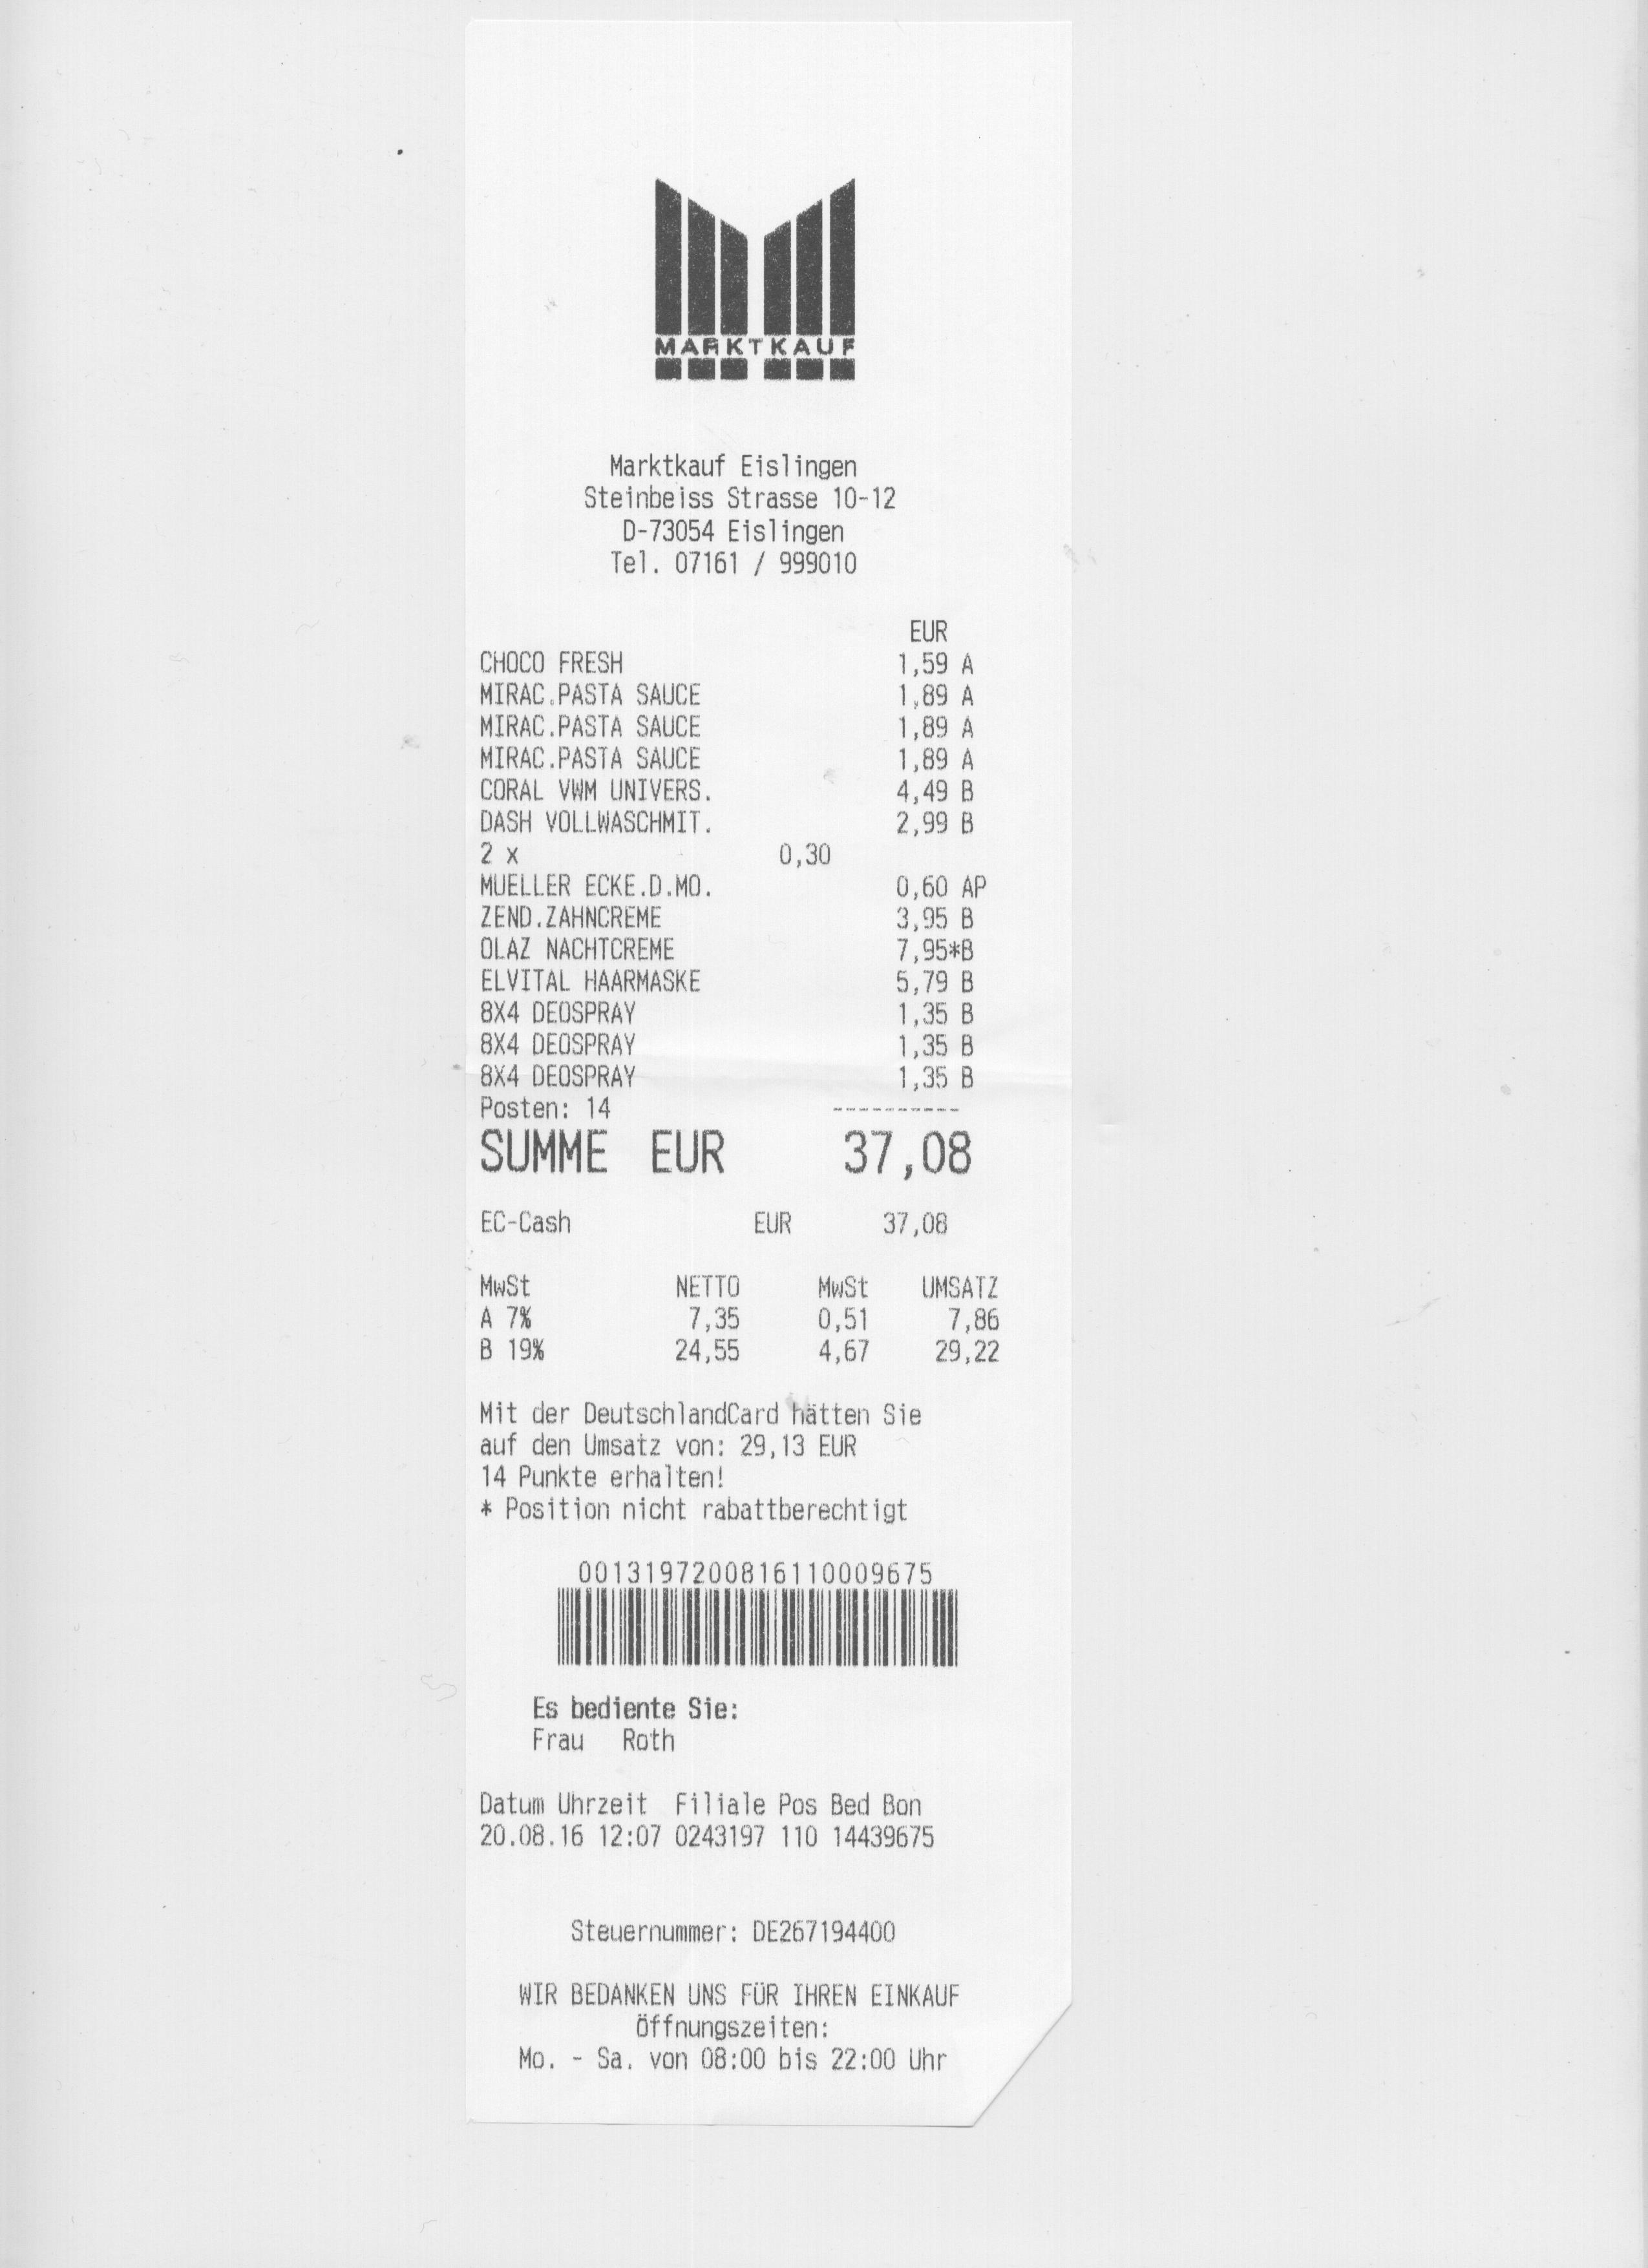
\includegraphics[width=100px]{images/001.jpg}}
\caption{This is an image from a text that uses color to teach music.}
\label{fig}
\end{figure}

\section[Auswertung und Analyse]{Auswertung und Analyse}

\lipsum[2]

Hier wird eine Quelle zitiert \cite{Quelle}.

\begin{thebibliography}{999}
\bibitem{Quelle} Versuchsanleitung zu (Abgerufen am 1.04.2050) 
\end{thebibliography}

% Für Dokumente mit mehr Referenzen empfiehlt es sich, auf eine separate .bib -Datei umzusteigen, die alle Referenzen enthält. Diese Referenzen können bei den meisten wissenschaftlichen Publikationen direkt über "BibTex-Export" oder ähnliches heruntergeladen werden. Anstelle von \begin{thebibliography}...\bibitem{}..\bibitem{}..\end{thebibliography} muss dann lediglich \bibliography{Dateiname.bib} eingebunden werden.

%\section{Anhang}
%\includepdf[pages=-]{Dateiname.pdf}


\end{document}